% WORKING DRAFT: for private review and revision, not an arXiv submission.
% Coauthors: please confirm order, affiliations, contact addresses, and contributions.
% TODO: Complete the priority check. Novelty of the lattice class results is unresolved.
% Format follows illumination-k4-codex/preprint-review-codex/revised.tex (preprint v0.2).
% Build: lualatex triangle-preprint.tex (twice).
\documentclass[11pt]{article}
\usepackage[T1]{fontenc}
\usepackage{lmodern}
\usepackage{amsmath,amssymb,amsthm,mathtools}
\usepackage{microtype}
\usepackage{geometry}
\geometry{letterpaper,margin=.9in}
\usepackage{tikz}
\usetikzlibrary{arrows.meta,calc}
\usepackage{hyperref}
\hypersetup{colorlinks=true,linkcolor=black,citecolor=black,urlcolor=blue!45!black}
\usepackage{enumitem}
\setlist[itemize]{nosep,leftmargin=1.5em}
\setlist[enumerate]{nosep,leftmargin=1.8em}
\setlength{\parindent}{0pt}
\setlength{\parskip}{3pt plus 1pt minus 1pt}
\allowdisplaybreaks
\definecolor{piecezero}{HTML}{F2E8D8}
\definecolor{pieceone}{HTML}{DCEAF2}
\definecolor{piecetwo}{HTML}{DDEDE5}
\definecolor{outline}{HTML}{233847}
\definecolor{seam}{HTML}{C78143}
\definecolor{markcolor}{HTML}{B84442}
\newtheorem{theorem}{Theorem}
\newtheorem{lemma}{Lemma}
\newtheorem{proposition}{Proposition}
\theoremstyle{remark}
\newtheorem{remark}{Remark}

\title{Illumination in three-star triangle rooms\\of surplus four}
\author{Daniel Wang\\\small Citizen Health \and Peyton Wang\\\small Francis Parker High School}
\date{Working draft v0.1 for discussion --- 6 November 2026\\\small Not submitted or peer reviewed}

\begin{document}
\maketitle
\vspace{-1.2em}
\begin{abstract}
A canonical triangle room is a strictly simple union of $45^\circ$--$45^\circ$--$90^\circ$ lattice tiles.
This note studies such rooms with interior even lattice points exactly $(0,0)$, $(2,0)$, and $(2,2)$.
Assume that the room has weighted surplus 4, at most 21 walls, and at most 6 transparent lattice points. This note proves that $(0,0)$ then illuminates $(2,2)$ within 32 reflections.
The theorem has no locality hypothesis.
The note gives the counting and structural reductions in full and summarizes the optical case proofs, which rely on exact certificates.
Independent AI review accepts the whole proof map, but no external referee or formal system has checked it.
Historical novelty is unresolved.
\end{abstract}

\section{Introduction}
A light ray in a polygonal room travels in a straight line and reflects specularly at smooth boundary points. A ray that reaches a corner stops. Two points \emph{illuminate} each other if a finite trajectory joins them.

Tokarsky constructed rooms with pairs that don't illuminate each other \cite{Tokarsky1995}. Lelièvre, Monteil, and Weiss \cite[Theorem~2]{LMW2016} and Wolecki \cite[Theorem~1.2(i)]{Wolecki2024} prove finiteness theorems for exceptional points and pairs. These theorems don't decide whether a specified pair illuminates. This note decides that question for one fixed configuration in a lattice class.

Tile the plane by splitting each unit square along the diagonal that joins an even-even point, type $A$, to an odd-odd point, type $B$. The third vertex of each tile has mixed parity, type $C$. Each tile has angles $45^\circ$ at $A$ and $B$ and $90^\circ$ at $C$.

A \emph{room} $R$ is a finite edge-to-edge union of tiles that is a closed disk with a strictly simple boundary. It has no holes, slits, pinches, or self-contacts. Define the following quantities:
\begin{itemize}
\item $W$: the number of maximal straight walls, which equals the number of corners.
\item $I$: the number of interior $A$ points. Each has a full \emph{star} of eight tiles.
\item $J$ and $s_N$: the numbers of interior and smooth-boundary points of type $B$ or $C$.
\item $k=J+s_N$: the number of \emph{transparent} points. These don't stop a ray.
\item $s_A$: the number of smooth-boundary $A$ points.
\item $Q=3s_A+\sum m$: the sum runs over $A$ corners, and $m$ counts the tiles at that corner.
\item $\Delta=Q+s_N-8$: the \emph{surplus}.
\end{itemize}

\begin{theorem}\label{thm:main}
Let $R$ be a room whose interior $A$ points are exactly $S=(0,0)$, $U=(2,0)$, and $T=(2,2)$. If $\Delta=4$, $W\le21$, and $k\le6$, then $R$ has a corner-avoiding specular trajectory from $S$ to $T$ with at most 32 reflections.
\end{theorem}

\begin{figure}[ht]
\centering
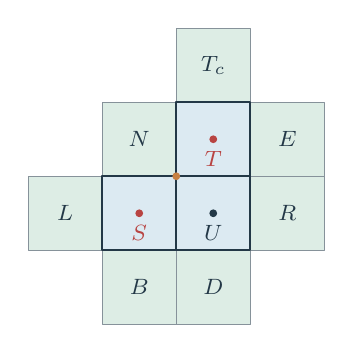
\begin{tikzpicture}[scale=.47,line join=round]
\foreach \x/\y/\n in {-2/0/L,0/-2/B,2/-2/D,4/0/R,4/2/E,2/4/{T_c},0/2/N}{
  \fill[piecetwo] (\x-1,\y-1) rectangle (\x+1,\y+1);
  \draw[outline!55,line width=.4pt] (\x-1,\y-1) rectangle (\x+1,\y+1);
  \node[font=\footnotesize,outline] at (\x,\y) {$\n$};
}
\foreach \x/\y in {0/0,2/0,2/2}{
  \fill[pieceone] (\x-1,\y-1) rectangle (\x+1,\y+1);
  \draw[outline,line width=.7pt] (\x-1,\y-1) rectangle (\x+1,\y+1);
}
\fill[markcolor] (0,0) circle (3pt) node[below=1pt,font=\footnotesize] {$S$};
\fill[outline] (2,0) circle (3pt) node[below=1pt,font=\footnotesize] {$U$};
\fill[markcolor] (2,2) circle (3pt) node[below=1pt,font=\footnotesize] {$T$};
\fill[seam] (1,1) circle (3pt);
\end{tikzpicture}
\qquad
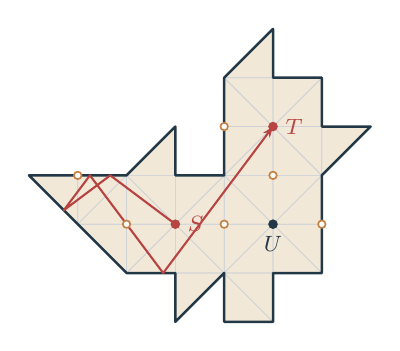
\begin{tikzpicture}[scale=.62,line join=round]
\fill[piecezero] (-3,1)--(-1,-1)--(0,-1)--(0,-2)--(1,-1)--(1,-2)--(2,-2)--(2,-1)--(3,-1)--(3,1)--(4,2)--(3,2)--(3,3)--(2,3)--(2,4)--(1,3)--(1,1)--(0,1)--(0,2)--(-1,1)--cycle;
\draw[outline!22,line width=.25pt] (-3,1)--(-2,0)--(-2,1)--cycle; \draw[outline!22,line width=.25pt] (-2,0)--(-2,1)--(-1,1)--cycle; \draw[outline!22,line width=.25pt] (-2,0)--(-1,-1)--(-1,0)--cycle; \draw[outline!22,line width=.25pt] (-2,0)--(-1,0)--(-1,1)--cycle; \draw[outline!22,line width=.25pt] (-1,-1)--(-1,0)--(0,0)--cycle; \draw[outline!22,line width=.25pt] (-1,-1)--(0,-1)--(0,0)--cycle; \draw[outline!22,line width=.25pt] (-1,0)--(-1,1)--(0,0)--cycle; \draw[outline!22,line width=.25pt] (-1,1)--(0,0)--(0,1)--cycle; \draw[outline!22,line width=.25pt] (-1,1)--(0,1)--(0,2)--cycle; \draw[outline!22,line width=.25pt] (0,-2)--(0,-1)--(1,-1)--cycle; \draw[outline!22,line width=.25pt] (0,-1)--(0,0)--(1,-1)--cycle; \draw[outline!22,line width=.25pt] (0,0)--(0,1)--(1,1)--cycle; \draw[outline!22,line width=.25pt] (0,0)--(1,-1)--(1,0)--cycle; \draw[outline!22,line width=.25pt] (0,0)--(1,0)--(1,1)--cycle; \draw[outline!22,line width=.25pt] (1,-2)--(1,-1)--(2,-2)--cycle; \draw[outline!22,line width=.25pt] (1,-1)--(1,0)--(2,0)--cycle; \draw[outline!22,line width=.25pt] (1,-1)--(2,-2)--(2,-1)--cycle; \draw[outline!22,line width=.25pt] (1,-1)--(2,-1)--(2,0)--cycle; \draw[outline!22,line width=.25pt] (1,0)--(1,1)--(2,0)--cycle; \draw[outline!22,line width=.25pt] (1,1)--(1,2)--(2,2)--cycle; \draw[outline!22,line width=.25pt] (1,1)--(2,0)--(2,1)--cycle; \draw[outline!22,line width=.25pt] (1,1)--(2,1)--(2,2)--cycle; \draw[outline!22,line width=.25pt] (1,2)--(1,3)--(2,2)--cycle; \draw[outline!22,line width=.25pt] (1,3)--(2,2)--(2,3)--cycle; \draw[outline!22,line width=.25pt] (1,3)--(2,3)--(2,4)--cycle; \draw[outline!22,line width=.25pt] (2,-1)--(2,0)--(3,-1)--cycle; \draw[outline!22,line width=.25pt] (2,0)--(2,1)--(3,1)--cycle; \draw[outline!22,line width=.25pt] (2,0)--(3,-1)--(3,0)--cycle; \draw[outline!22,line width=.25pt] (2,0)--(3,0)--(3,1)--cycle; \draw[outline!22,line width=.25pt] (2,1)--(2,2)--(3,1)--cycle; \draw[outline!22,line width=.25pt] (2,2)--(2,3)--(3,3)--cycle; \draw[outline!22,line width=.25pt] (2,2)--(3,1)--(3,2)--cycle; \draw[outline!22,line width=.25pt] (2,2)--(3,2)--(3,3)--cycle; \draw[outline!22,line width=.25pt] (3,1)--(3,2)--(4,2)--cycle;
\draw[outline,line width=.9pt] (-3,1)--(-1,-1)--(0,-1)--(0,-2)--(1,-1)--(1,-2)--(2,-2)--(2,-1)--(3,-1)--(3,1)--(4,2)--(3,2)--(3,3)--(2,3)--(2,4)--(1,3)--(1,1)--(0,1)--(0,2)--(-1,1)--cycle;
\draw[markcolor,line width=.75pt,-{Stealth[length=4pt]}] (0,0)--(-4/3,1)--(-16/7,2/7)--(-7/4,1)--(-1/4,-1)--(2,2);
\foreach \p in {(-2,1),(-1,0),(1,0),(1,2),(2,1),(3,0)} \draw[seam,fill=white,line width=.6pt] \p circle (2.2pt);
\fill[markcolor] (0,0) circle (2.8pt) node[right=1pt,font=\footnotesize] {$S$};
\fill[outline] (2,0) circle (2.8pt) node[below=1pt,font=\footnotesize] {$U$};
\fill[markcolor] (2,2) circle (2.8pt) node[right=1pt,font=\footnotesize] {$T$};
\end{tikzpicture}
\caption{Left: the core $H$ (blue) and its seven neighboring $A$ cells (green), which together form $K$. The orange dot marks $(1,1)$. Right: a qualifying room with 34 tiles, $W=20$, $J=s_N=3$, $k=6$, and $Q=9$. Open circles mark transparent points. The path $S\to(-\tfrac43,1)\to(-\tfrac{16}7,\tfrac27)\to(-\tfrac74,1)\to(-\tfrac14,-1)\to T$ has four reflections. It crosses the transparent point $(-1,0)$.}
\label{fig:room}
\end{figure}

\begin{remark}
The pairs $(S,U)$ and $(U,T)$ have direct segments, so the theorem covers every pair of interior $A$ points in $R$. It doesn't address other points, other supports, other surpluses, or arbitrary polygons. It isn't a universal minimum on walls.
\end{remark}

\paragraph{Related work.} De Winter and Tokarsky study lattice rooms whose tile vertices are corners \cite{DeWinterTokarsky2026}. This note instead allows transparent points. The authors' working note \cite{WangWang2026} gives a strictly simple orthogonal 22-wall room with a dark pair.

An unpublished computer-assisted theorem of the same project uses SAT refutations. It states that all pairs of interior $A$ points illuminate when $W\le21$ and $k\le6$. That theorem already contains the existence part of Theorem~\ref{thm:main}. This note adds a case proof with no SAT refutation in its source manifest, and an explicit reflection bound. The project's literature check found no antecedent, but novelty remains unresolved.

\section{Counting}\label{sec:counting}
\begin{lemma}\label{lem:count}
Every room satisfies $W=2+6I+Q-2J-s_N$. If $I=3$, then $W+2k=28+\Delta$.
\end{lemma}
\begin{proof}
Let $N$ be the number of tiles. Euler's formula for the triangulated disk gives $N=2(I+J)+W+s_A+s_N-2$. Each tile has one $A$ vertex, so $N=8I+Q+s_A$, because a smooth $A$ point has four tiles and weight 3. Subtract these equations. For $I=3$, substitute $Q=\Delta+8-s_N$.
\end{proof}
So under the hypotheses of Theorem~\ref{thm:main}, $W+2k=32$. The bounds force $W=20$ and $k=6$.

The \emph{cell} of an $A$ point is the square of side 2 centered at it. Let $H$ be the union of the stars of $S$, $U$, and $T$. Its boundary has 8 exposed cell sides. Each is shared with one of the seven neighboring cells $L=(-2,0)$, $B=(0,-2)$, $D=(2,-2)$, $R=(4,0)$, $E=(4,2)$, $T_c=(2,4)$, and $N=(0,2)$. The cell $N$ has two exposed sides. Let $K$ be $H$ with those seven cells. A cell outside $K$ is \emph{remote}.

Each cell side has two $BC$ edges, which meet at a $C$ midpoint. An occupied non-full cell $v$ is a contiguous fan of $m(v)$ tiles, because the boundary is strictly simple. Set $q(v)=m(v)$, except $q(v)=3$ for a smooth four-tile half-star. Let $d(v)$ count the exposed sides that $v$ touches, and set $e(v)=q(v)-d(v)\ge0$. Let $M$ be the set of $C$ midpoints of untouched exposed sides. Each is a smooth boundary point. Set $b=s_N-|M|\ge0$.

\begin{lemma}[Charge identity]\label{lem:charge}
$\Delta=\sum_v e(v)+b$.
\end{lemma}
\begin{proof}
Here $Q=\sum_v q(v)$, and the exposed sides give $8=\sum_v d(v)+|M|$. Substitute both into $\Delta=Q+s_N-8$.
\end{proof}

\section{Structural reduction}\label{sec:structure}
Each tile has one $BC$ edge, and that edge lies on a cell side. So the occupied cells form a connected graph under shared $BC$ edges. Number the tiles of the cell $N$ cyclically, so that tiles 6 and 7 meet at $(1,1)$. If both are present, then $(1,1)$ is interior, and the segment $ST$ lies in $R$. Exclude this \emph{bridge} from now on.

A \emph{centered pair} is two tiles that share an $AC$ edge. It fills $180^\circ$ at $C$, and both of its $BC$ edges lie on one side. A \emph{quarter pair} is two tiles that share an $AB$ edge. It contributes $90^\circ$ at the $C$ midpoints of two different sides. A cell with $d>0$ is a \emph{root}.

The following facts hold without the bridge:
\begin{enumerate}[label=(F\arabic*)]
\item Only $N$ can have $d=2$. A fan that meets both sides of $N$ contains the bridge, unless it has at least six tiles and $e\ge4$. That excess leaves no charge for another positive cell.
\item No cell has $q=4$, because a four-tile fan is a smooth half-star with $q=3$.
\item A cell with $e=0$ is a single tile whose only $BC$ edge faces $H$. It can't connect $H$ to another cell.
\item A root with $e=1$ is a centered pair with no outward side, or a quarter pair with one outward side.
\item A cell with $d=0$ and $e=1$ is a single tile. It has one $BC$ edge, so it is a leaf of the graph.
\item A cell with $d=0$, $e=2$, and two neighbors is a quarter pair.
\item At a $C$ point outside $H$, only the two adjacent $A$ cells contribute tiles. Two $90^\circ$ contributions form a smooth $C$ point and add 1 to $b$. No third cell can change that.
\end{enumerate}

\begin{proposition}\label{prop:structure}
Assume the hypotheses of Theorem~\ref{thm:main} and no bridge.
\begin{enumerate}
\item At most one cell is remote. If one exists, it shares an edge with a unique root in $K$.
\item Without a remote cell, $(e\text{-parts};b)$ has one of ten types: $b4$, $e1{+}b3$, $e2{+}b2$, $2e1{+}b2$, $e2{+}e1{+}b1$, $3e1{+}b1$, $e3{+}e1$, $2e2$, $e2{+}2e1$, and $4e1$.
\item With a remote cell, let $r$, $l$, and $h$ be the excess of the parent, the remote cell, and the other cells. Then $(r,l,h,b)$ is one of $(1,1,0,2)$, $(1,2,0,1)$, $(1,3,0,0)$, $(1,1,1,1)$, $(1,2,1,0)$, $(2,1,0,1)$, $(2,2,0,0)$, and $(2,1,1,0)$.
\end{enumerate}
\end{proposition}
\begin{proof}
\emph{Part 1, two remote cells.} Suppose that two cells are remote, and take a tree in the cell graph that connects $H$ to both. By (F3), each cell in the tree has positive excess, and Lemma~\ref{lem:charge} gives $\sum e\le4$. With three positive cells, (F4), (F5), and (F6) leave two patterns.
\begin{itemize}
\item A root with $e=2$ has two leaves with $e=1$. By (F1), the root has $d=1$ and $q=3$, so it must meet three sides. Three tiles meet at most two sides. Four tiles meet three sides with contributions $90^\circ$, $180^\circ$, and $90^\circ$. At most one side faces $H$, so one leaf joins a $90^\circ$ contribution. Then (F7) gives $\sum e+b\ge5$.
\item A root with $e=1$ connects through a remote quarter pair with $e=2$ to a leaf with $e=1$. This chain forms two smooth $C$ points, so $\sum e+b\ge6$.
\end{itemize}
With four positive cells, each has $e=1$. All cells with $d=0$ are leaves, and a root has at most one neighbor outside $H$. So two remote leaves need two roots. Each pair forms a smooth $C$ point, so $\sum e+b\ge6$. Adjacencies outside the tree can't repair these points, by (F7). Each case contradicts $\Delta=4$.

\emph{Part 1, one remote cell.} An intermediate cell with $d=0$ must pass the connection onward. The shortest such chain is the second pattern, which is excluded. So the remote cell is adjacent to a root in $K$. Two roots need $q\ge2$ at the remote cell. The only choice within charge 4 is two roots with $e=1$ and a remote quarter pair with $e=2$. Its two joins force $b\ge2$, which exceeds the charge.

\emph{Part 2.} The value of $b$ and a partition of $4-b$ give twelve weighted partitions. Two of them are impossible. In a sole $e3{+}b1$, the only positive cell must touch $H$, by (F3). Then $d=1$ needs $q=4$, and $d=2$ needs a five-tile fan that contains the bridge. In a sole $e4$ with $d=1$, the five-tile fan has at least two centered pairs, and only one faces $H$. The other forms a smooth $C$ point, which contradicts $b=0$. With $d=2$, the only fan is the six-tile window of tiles 0 through 5 in $N$. Its two centered pairs outside $H$ form smooth $C$ points, and no charge remains to repair them.

\emph{Part 3.} Here $r,l\ge1$. By (F1) and (F2), $r=3$ and $l=4$ are impossible. A join with $r=l=1$ forms a smooth $C$ point by (F4), (F5), and (F7), so it has $b\ge1$. That excludes $(1,1,2,0)$. The remaining solutions of $r+l+h+b=4$ are the eight rows.
\end{proof}

Parts 2 and 3 are necessary lists. A listed type needn't contain a valid room.

\section{Guards and erasure}\label{sec:guards}
A \emph{guard} for an exact rational path $\gamma$ from $S$ to $T$ is a pair $(\mathcal U,\mathcal Z)$ of tile sets. The set $\mathcal U$ contains every tile that $\gamma$ needs. It includes the full star of each lattice point on an open leg. It also includes the connected $180^\circ$ sector of each smooth contact at a lattice point. The set $\mathcal Z$ contains the tile across each mirror contact.

\begin{lemma}[Guards]\label{lem:guard}
If $\mathcal U\subseteq R$ and $R\cap\mathcal Z=\emptyset$, then $\gamma$ is a legal trajectory in $R$. The map $\sigma(x,y)=(2-y,2-x)$ with reversal fixes $U$, exchanges $S$ and $T$, and sends guards to guards.
\end{lemma}
\begin{proof}
The set $\mathcal U$ keeps each leg in $R$ and keeps each crossed lattice point interior. The set $\mathcal Z$ makes each contact a boundary point. The map $\sigma$ is the reflection in $x+y=2$, which preserves the tiling and $K$.
\end{proof}

Enlarging a room can remove a mirror, so illumination isn't monotone under enlargement. All transfer arguments in this note preserve a guard. They don't assume monotonicity.

\begin{proposition}[Unit theorems]\label{prop:unit}
Let $R$ lie in $K$ with full stars exactly $S$, $U$, and $T$. Suppose that every non-full cell has $e=0$, except for at most two cells with $e=1$. Then $S$ illuminates $T$ within 13 reflections. The selected guards lie in $K$. The result has no hypothesis on $b$, $W$, or $k$.
\end{proposition}

This note doesn't reproduce the proof. It uses 21 fixed building-block paths with their $\sigma$-images and exchanges at critical cells. Each exchange keeps its entry and exit states and stays in $K$.

\begin{proposition}[Erasure and restoration]\label{prop:erasure}
In each of the five rows with $r=1$, $S$ illuminates $T$ within 13 reflections.
\end{proposition}
\begin{proof}
The parent is a quarter pair with one outward $BC$ edge. By unique parenthood and fan geometry, the remote fan meets the rest of $R$ along that edge and its endpoints. In the rows with $h=1$, the extra unit cell remains a root. A remote single tile has no unused $BC$ edge. A remote pair with $b=0$ must be centered toward its parent, so it has no onward edge either. Delete the remote fan, which is a disk glued along one boundary edge. The result is a strictly simple disk in $K$, with the same full stars and at most two cells of excess 1. The budgets $\Delta$, $b$, $W$, and $k$ needn't persist, and the proof doesn't use them. Proposition~\ref{prop:unit} gives a path whose guard lies in $K$. Restoring the remote fan changes neither $\mathcal U$ nor $\mathcal Z$.
\end{proof}

\section{Case closure and proof of Theorem~\ref{thm:main}}\label{sec:closure}
Table~\ref{tab:cases} lists the proved bound for each type. The bound 32 comes from two fixed residual rooms of type $e2{+}b2$, whose paths start in direction $(-20,-9)$. It is conservative and isn't known to be sharp.

\begin{table}[ht]
\centering
\small
\begin{tabular}{llcl}
\hline
Branch & Type or row & Bound & Method\\
\hline
Local & $b4$ & 13 & Proposition~\ref{prop:unit}\\
 & $e1{+}b3$ & 13 & Proposition~\ref{prop:unit}\\
 & $e2{+}b2$ & 32 & Single-excess-2 closure, with two fixed rooms at 32\\
 & $2e1{+}b2$ & 13 & Proposition~\ref{prop:unit}\\
 & $e2{+}e1{+}b1$ & 14 & Root and leaf cover, with critical cells separate\\
 & $3e1{+}b1$ & 13 & Separate three-unit proof\\
 & $e3{+}e1$ & 13 & Root and leaf cover in $K$\\
 & $2e2$ & 19 & Joined-cell proof\\
 & $e2{+}2e1$ & 13 & Leaf, root, and critical-cell covers\\
 & $4e1$ & 13 & Erasure, or a cover of 208 symbolic labels\\
\hline
Remote & Five rows with $r=1$ & 13 & Proposition~\ref{prop:erasure}\\
 & $(2,2,0,0)$ & 23 & Whole-row proof\\
 & $(2,1,0,1)$ & 13 & 18 necessary interfaces and 205 labels\\
 & $(2,1,1,0)$ & 13 & 44 necessary interfaces, each with a full guard\\
\hline
\end{tabular}
\caption{Reflection bounds for all cases of Proposition~\ref{prop:structure}.}
\label{tab:cases}
\end{table}

\begin{proof}[Proof of Theorem~\ref{thm:main}]
If the bridge is present, the segment $ST$ works. Otherwise, Proposition~\ref{prop:structure} places $R$ in one row of Table~\ref{tab:cases}. Each row has a path of the stated length, with a guard that $R$ satisfies. The largest bound is 32.
\end{proof}

This note doesn't reproduce the optical case proofs behind Table~\ref{tab:cases}. The source manifest pins 148 files across these proofs, their reviews, and their checkers.

\section{Verification status}\label{sec:status}
\paragraph{Checks.} The exact checker recomputes 436 necessary interface patches, 2{,}546 angular completions, and the guards of the 21 building-block paths, including reversal and $\sigma$. These are local checks, not a count of rooms. The archived verification records report matching 148 manifest pins, 6 supplement pins, and 157 review pins.

\paragraph{Limits.} Some checks rely on shared lower-layer foundations, so their independence is limited. Some optical paths came from earlier bounded searches; the proof uses each path only through its exact guard. Computational replay is not a fresh hand proof of every inherited lemma. No proof assistant or external expert has checked the result.

\paragraph{Data availability.} The proof records, exact checkers and certificate download instructions are in the project repository: \url{https://github.com/peytonprogrammer/illumination-problem}. See \texttt{docs/DATA.md} and \texttt{docs/REPRODUCIBILITY.md}. Access follows the repository policy; this draft does not claim a public supplement.

\paragraph{Open questions.} Lemma~\ref{lem:count} also allows $\Delta=5$ with $W=21$ and $k=6$, which this theorem doesn't cover. Other three-star supports are also outside it. It's open whether a bound below 32 holds.

\section*{Acknowledgments}
The authors used AI tools, including OpenAI Codex and Anthropic Claude, to develop and revise this research, its theorem proofs, and the manuscript. The authors remain responsible for the content.

\begin{thebibliography}{9}
\bibitem{DeWinterTokarsky2026}
J.~de~Winter and G.~W. Tokarsky, ``Unilluminable rooms: minimal examples, classifications and exceptions,''
manuscript, 31 October 2026.
\url{https://github.com/JoostdeWinter/unilluminable-rooms/blob/main/unilluminable_rooms.tex}.

\bibitem{LMW2016}
S.~Lelièvre, T.~Monteil, and B.~Weiss, ``Everything is illuminated,''
\emph{Geometry \& Topology} \textbf{20} (2016), 1737--1762.
\url{https://arxiv.org/abs/1407.2975}.

\bibitem{Tokarsky1995}
G.~W. Tokarsky, ``Polygonal rooms not illuminable from every point,''
\emph{The American Mathematical Monthly} \textbf{102} (1995), no.~10, 867--879.
\url{https://doi.org/10.1080/00029890.1995.12004679}.

\bibitem{WangWang2026}
D.~Wang and P.~Wang, ``A simple orthogonal 22-gon with two non-illuminating interior points,''
working draft v0.2, 2 November 2026. Not submitted.

\bibitem{Wolecki2024}
A.~Wolecki, ``Illumination in rational billiards,''
\emph{arXiv:1905.09358v3} (2024).
\url{https://arxiv.org/abs/1905.09358v3}.
\end{thebibliography}
\end{document}
